\documentclass[a4paper,12pt]{article}
%\documentclass[a4paper,10pt]{scrartcl}

\usepackage{scrextend}
\changefontsizes[14pt]{14pt}

\usepackage[T1]{fontenc}
\usepackage{lmodern}
\usepackage[utf8x]{inputenc}
\usepackage{graphicx}
\usepackage{tabularx}
\usepackage{multirow}
\usepackage{booktabs}
\usepackage{colortbl}
\usepackage[italian]{babel}
\usepackage[margin=2cm]{geometry}
\usepackage{color}
\definecolor{mygrey}{gray}{0.4}
\definecolor{light-blue}{rgb}{0.4,0.5,1}
\definecolor{light-cyan}{rgb}{0.4,0.6,1}
\usepackage{booktabs}

%Header and footer of pages
\usepackage{fancyhdr}
\pagestyle{fancy}
\lhead{\textcolor{mygrey}{Emanuele Uliana, Gabriele Rufolo, Walter Rubino}}
\rhead{\textcolor{mygrey}{Manuale di installazione}}

%Set paragraphs indentation to 0 points
\setlength{\parindent}{0pt}

%Sections and subsections' style
\usepackage{titlesec} 
\titleformat{\section} {\color{blue}\normalfont\sffamily\Large\bfseries} {\color{blue}\thesection}{20pt}{} 
\usepackage{titlesec}
\titleformat{\subsection} {\color{light-blue}\normalfont\sffamily\large\bfseries\itshape} {\color{light-blue}\thesubsection}{18pt}{} 
\titleformat{\subsubsection} {\color{light-cyan}\normalfont\sffamily\large\bfseries\itshape} {\color{light-cyan}\thesubsubsection}{14pt}{} 



%Document default font family
\renewcommand{\familydefault}{\sfdefault}
\renewcommand*\arraystretch{1.5}

\pdfinfo{%
  /Title    (SWIMv2 - Manuale di installazione)
  /Author  (Emanuele Uliana /and Gabriele Rufolo / and Walter Rubino)
  /Creator  (Emanuele Uliana /and Gabriele Rufolo / and Walter Rubino)
  /Producer (Emanuele Uliana /and Gabriele Rufolo / and Walter Rubino)
  /Subject  (Manuale d'uso)
  /Keywords ()

}

\begin{document}
\vspace*{\fill}
\begin{center}
{\fontsize{28}{10} \selectfont \textcolor{mygrey}{Progetto di Ingegneria del Software 2} \\[2\baselineskip]} {\fontsize{42}{10} \selectfont {\bfseries SWIMv2}} \\[4\baselineskip]

\includegraphics[scale=1]{wave-icon} \\[4\baselineskip]
{\fontsize{28}{10} \selectfont {\bfseries \textcolor{blue}{Manuale d'uso}} \\[2\baselineskip] A.A. 2012/2013}
\end{center}
\begin{flushleft}
{\fontsize{18}{10}
{\bfseries Autori}: \\ Emanuele Uliana (799256), Gabriele Rufolo (743695), Walter Rubino (742519) \\[1\baselineskip]
{\bfseries Docente}: \\ Prof.ssa Raffaela Mirandola
}
\end{flushleft}
\vspace*{\fill}
\begin{center}
Versione 1.0 del 26/1/2013 \\
\end{center}

\clearpage

	    \vspace*{\fill}
	\tableofcontents
	    \vspace*{\fill}

\clearpage

\section{Introduzione}
Questo documento si propone di essere un semplice manuale di installazione per tester del progetto SWIMv2. Alcuni dettagli sono descritti nel manuale d'uso, in quanto più attinenti
ad esso.

\section{Prerequisiti software}
\begin{itemize}
 \item Occorre aver installato e configurato correttamente JBoss AS 5.1.0
 \item Gli altri prerequisiti sono descritti più dettagliatamente nel manuale d'uso
\end{itemize}

\section{Installazione vera e propria}
Occorre procedere per gradi

\subsection{Configurazione del server affinche' accetti solo connessioni in https}
Nel file path\_di\_installazione\_di\_jboss/server/default/deploy/jbossweb.sar/server.xml  commentate le seguenti righe:

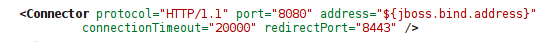
\includegraphics[scale=0.8]{linestocomment}

e decommentate le seguenti, modificandole, nel caso fossero diverse, rendendole coincidenti con quelle qui sotto:

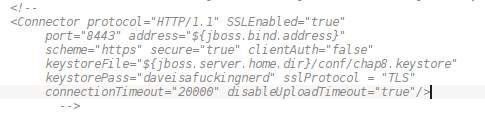
\includegraphics[scale=0.8]{linestouncomment}

Inoltre occorre prendere il file chap8.keystore dalla cartella utilities e metterlo in  path\_di\_installazione\_di\_jboss/server/default/conf/

Molto importante è il fatto che, per un corretto funzionamento, il server deve essere lanciato da terminale e NON da Eclipse: se usate Mac OS X o un sistema GNU/Linux saprete bene
come avviare un terminale, mentre da Windows è necessario cercare dal menù start il file cmd.exe ed eseguirlo. A questo punto date il seguente comando:

cd path\_di\_installazione\_di\_jboss/bin/

e a questo punto da Mac/Linux date ./run.sh , mentre da Windows date run.bat

\subsection{Creazione di un database MySql e configurazione del server per connettersi ad esso}
\begin{itemize}
 \item Create un database MySql esattamente di nome SWIMv2\_DB
 \item Prendete dalla cartella utilities il file database-ds.xml e mettetelo nel seguente percorso: (path di installazione di jboss)/server/default/deploy/   supponendo che usiate il
 server di default
 \item Eventualmente date i permessi di accesso a quel file e al database (in ambiente GNU/Linux un chmod 777, per quanto troppo permissivo, risolve qualunque problema, o quasi)
\end{itemize}

\subsection{Copia dei file del progetto nella cartella deploy del server}
Prendete dalla cartella utilities i file SWIMv2\_DWP.war e SWIMv2\_EJB.ear e mettete anch'essi nella cartella deploy del server.

\end{document}